\documentclass[addpoints,12pt]{exam}
\newcommand{\ds}{\displaystyle}
\usepackage[margin=0.8in]{geometry}
\usepackage{subcaption}
\usepackage{tikz}
\usepackage{amssymb,amsmath,graphicx,wrapfig,verbatim,wasysym, enumitem,psfragx,color}
\usepackage{multicol}

%\usepackage{fancyhdr}
%\setlength{\headheight}{13.6pt}
%\pagestyle{fancy}
%\lhead{Math 222}
%\chead{ Midterm 1 }
%\rhead{Spring 2022}

\def\FillInBlank{\rule{3truein} {.01truein}}


% Choose one option (bubbles)
\newcommand{\chooseone}{{\Large$\Circle$\ \ }}


\newcommand{\myleft}{\makebox[.4\textwidth]{First Name:\enspace\hrulefill}}
\newcommand{\myright}{\makebox[.4\textwidth]{Last Name:\enspace\hrulefill}}
\header{\oddeven{\myleft}{}}
    {}
    {\oddeven{\myright}{}}

\footrule

\footer{Math 211}
     {Midterm 2 - Practice Exam}
     {Page \thepage\ of \numpages}

\begin{document}

\begin{questions}


\question Are each of the following true or false statements? Fill in the bubble next to the
correct answer. Justification is not necessary.


Reminder: Elasticity $=E(p)=\dfrac{-pD'(p)}{D(p)}$

\begin{parts}

\part[2] Suppose the demand function of a commodity is $D(p)=20-p$. If the current price is
$p=5$, the demand is elastic.

\begin{itemize}[label={}]
\item \chooseone True
\item \chooseone False
\end{itemize}

\vfill




\part[2] The value of $\$1000$ deposited in a bank at $12\%$ interest compounded quarterly for
15 years is $1000(1.03)^{15}$ dollars.

\begin{itemize}[label={}]
\item \chooseone True
\item \chooseone False
\end{itemize}

\vfill




%\part[2] For $y=5x^2$, the differential $dy$ at $x=2$ and $dx=0.3$ is $dy=6$.
%\begin{itemize}[label={}]
%\item \chooseone True
%\item \chooseone False
%\end{itemize}

%\vfill


\part[2] The function $f(x)=x^2-4x$ has an absolute minimum value of $-3$ on the interval
$[3,6]$.
\begin{itemize}[label={}]
\item \chooseone True
\item \chooseone False
\end{itemize}




\vfill

\end{parts}

\newpage

\question Use the given graph of the function $f$ to answer the following questions. Fill in the
bubble next to the correct answer. Justification is not necessary.

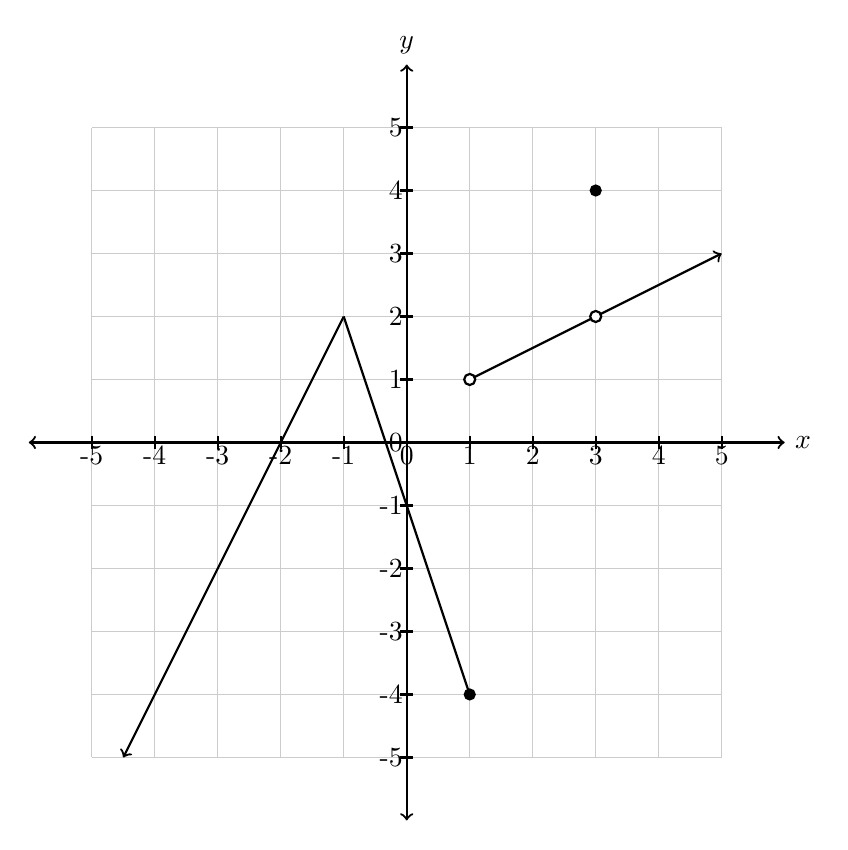
\begin{tikzpicture}[scale=.8]
\draw[gray!40] (-5, -5) grid[step=1] (5, 5);
\draw[<->,thick,black] (-6,0)--(6,0) node[right]{$x$};
\draw[<->, thick,black] (0,-6)--(0,6) node[above]{$y$};
\foreach \x in {-5,-4,...,5}
\draw[thick] (\x,-.1) --(\x,.1) node[below]{\x};
\foreach \y in {-5,-4,...,5}
\draw[thick] (-.1,\y) --(.1,\y) node[left] {\y};
\draw[domain=-4.5:-1,samples=100, thick,<-] plot ({\x},{2*(\x+1)+2});
\draw[domain=-1:1,samples=100, thick,-] plot ({\x},{-3*(\x+1)+2});
\draw[domain=1:5,samples=100,thick,->] plot ({\x},{(\x/2+0.5});
\draw[fill=black] (3,4) circle[radius=0.25em];
\draw[fill=black] (1,-4) circle[radius=0.25em];
\draw[fill=white,thick] (3,2) circle[radius=0.25em];
\draw[fill=white,thick] (1,1) circle[radius=0.25em];
\end{tikzpicture}

\begin{parts}
\part[1] The function is not differentiable at $x = -2.$
\begin{itemize}[label={}]
\item \chooseone True
\item \chooseone False
\end{itemize}

\part[1] The function is not differentiable at $x = -1.$
\begin{itemize}[label={}]
\item \chooseone True
\item \chooseone False
\end{itemize}

\part[1] The function is not differentiable at $x = 0.$
\begin{itemize}[label={}]
\item \chooseone True
\item \chooseone False
\end{itemize}

\part[1] The function is not differentiable at $x = 1.$
\begin{itemize}[label={}]
\item \chooseone True
\item \chooseone False
\end{itemize}

\part[1] The function is not differentiable at $x = 3.$
\begin{itemize}[label={}]
\item \chooseone True
\item \chooseone False
\end{itemize}

\part[2] The given function is
\begin{itemize}[label={}]
\item \chooseone differentiable
\item \chooseone nondifferentiable
\item \chooseone neither
\end{itemize}

\end{parts}

\newpage


\question
 Let $f(x)$ be a continuous function with derivative $\ds f'(x)=(x-2)^2(x+3)(x-5)$.
\begin{parts}

\part[3] Give all critical numbers for $f(x)$.


\vspace{1.5in}


\part[7] Using a sign chart, find the intervals of increasing and decreasing for $f(x)$. Write your
answers using interval notation.

\vspace{4in}


\part[3] Classify each critical number as a relative minimum, relative maximum, or neither.

\end{parts}

\newpage


\question[10] On the axes below,
draw the graph of a continuous function $f(x)$ that satisfies the following:\smallskip

​      $f(0)=5$\smallskip
​
​      $f'(0)=0$ \smallskip
​
​      $f'(x)>0$ on $(-\infty, 0)$\smallskip
​
​      $f'(x)<0$ on $(0,\infty)$\smallskip
​
​
​      $f''(x)<0$ on $(-\infty, 2)$ \smallskip
​
​      $f''(x)>0$ on $(2,\infty)$\smallskip

$\ds\lim_{x\to\infty}f(x)=1$


​      \begin{tikzpicture}[scale=1]
​      \draw[gray!60] (-7, -7) grid[step=1] (7, 7);
​      \draw[<->, thick,black] (-8,0)--(8,0) node[right]{$x$};
​      \draw[<->, thick,black] (0,-8)--(0,8) node[above]{$y$};
​      \foreach \x in {-7,-6,...,7}
​      \draw[thick] (\x,-.1) --(\x,.1)node[below]{\x};
​      \foreach \y in {-7,-6,...,7}
​      \draw[thick] (-.1,\y) --(.1,\y)node[left]{\y};
​      \end{tikzpicture}
​
​

\newpage

\question[12]
​       Farmer Stan is building a rectangular cattle pen to be enclosed by a fence and divided
into three equal parts by two

​      additional fences parallel to one of the sides (see picture below). If he has 200 meters of
fencing available to use, what dimensions for the outer rectangle (i.e., what values for $x$ and
$y$) will create the largest possible total area? Justify that your solution is optimal. Show all
work.

\bigskip

​       \begin{figure}[h]
​       ​       \begin{center}
​       ​       ​       \begin{tikzpicture}
​       ​       ​       ​       \draw[thick] (0,0) -- (6,0)--(6,4)--(0,4)--(0,0);
​       ​       ​       ​       \draw[thick] (2,0) -- (2,4);
​       ​       ​       ​       \draw[thick] (4,0) --(4,4);
   \draw (0,4.2)--(6,4.2);
   \draw (0,4.1)--(0,4.3);
   \draw (6,4.1)--(6,4.3);
   \draw (6.2,0)--(6.2,4);
   \draw (6.1,0)--(6.3,0);
   \draw (6.1,4)--(6.3,4);
\draw (3,4.2) node[inner sep=2pt,fill=white] {$x$};
\draw (6.2,2) node[inner sep=2pt,fill=white] {$y$};
​       ​       ​       ​
​       ​       ​       ​
​       ​       ​       \end{tikzpicture}
​       ​       \end{center}
​       ​       %\caption{Useful figure for Problem 4}
​       \end{figure}

\newpage

\question[10] Find the intervals of concavity and inflection points ($x$ values only) of\\
$f(x)=\frac{1}{2}{x}^{4}-5{x}^{3}+12{x}^{2}+17x+89$. Give the intervals of concavity using
interval notation. Show all work.


\newpage




\question[12] An Etsy necklace maker finds that when they price their necklaces at $\$20 $, they
sell $100$ necklaces in a month. They determine that for each $\$1 $ price increase, they will
sell 4 fewer necklaces per month. If each necklace costs $\$5$ to produce, what price should
they charge to maximize profit? Justify your solution is optimal.

\newpage




\question


\begin{parts}

\part[6] After $t$ days of advertisements for a new restaurant, the proportions of shoppers in a
town who have seen the ads is $1-e^{-0.04t}.$ How long must the ads run to reach 90\% of the
shoppers? You do not need to simplify your answer.
%4.2


\vfill

\part[6] Find $\dfrac{d}{dt}\ln(f(t))$ (i.e. the relative rate of change) of $f(t)=t^2+1$ at $t=2$.

\vfill

\part[6] A car worth \$15,000 depreciates in value by 15\% each year. How much is it worth after
5 years? You do not need to simplify your answer.
%4.1

\vfill


\end{parts}

\newpage

\question Compute the following derivatives.

\begin{parts}

\part[6] Find $f'(x)$ if $f(x) = \ln(x) \sqrt{x}.$ You do not need to simplify your final answer.

\vfill

\part[6] Find $g''(x)$ if $g(x)=e^{x^3}$. You do not need to simplify your final answer.

\vfill

\end{parts}




\newpage




\end{questions}

\end{document}
